\documentclass[11pt,a4paper]{article}

\usepackage[top=1.8cm,bottom=1.8cm,left=2cm,right=2cm]{geometry}
\usepackage[T1]{fontenc}
\usepackage[utf8]{inputenc}
\usepackage[italian]{babel}
\usepackage{lmodern}
\usepackage{microtype}
\usepackage{graphicx}
\graphicspath{{figures/}}
\usepackage{booktabs}
\usepackage{amsmath}
\usepackage{float}
\usepackage{caption}
\usepackage{hyperref}
\usepackage{xurl}
\usepackage[round,authoryear]{natbib}

\hypersetup{colorlinks=true,linkcolor=black,citecolor=black,urlcolor=black}
\urlstyle{same}
\captionsetup{font=small,labelfont=bf,skip=5pt}
\setlength{\parindent}{0pt}
\setlength{\parskip}{3pt}
\setlength{\intextsep}{8pt plus 2pt minus 2pt}
\setlength{\textfloatsep}{10pt plus 2pt minus 2pt}
\emergencystretch=2em
\renewcommand{\refname}{Riferimenti bibliografici}

\begin{document}

\begin{center}
{\LARGE Il posizionamento competitivo delle imprese europee della filiera dei semiconduttori nell'era dell'AI: un'analisi comparativa (2021--2025)}

\vspace{0.7cm}
{\large Salvatore Megna}

\vspace{0.25cm}
Agosto 2026
\end{center}

\vspace{0.5cm}

\section{Introduzione e obiettivo dell'analisi}

Negli ultimi anni, la rapida diffusione dell'intelligenza artificiale ha aumentato la domanda di capacità di calcolo e rafforzato il ruolo dei semiconduttori avanzati nell'infrastruttura digitale. Lo sviluppo di processori, memorie e architetture sempre più complesse coinvolge non soltanto i produttori di chip, ma anche le imprese che forniscono le tecnologie necessarie alla loro fabbricazione, al packaging e al testing.

In Europa operano alcune società altamente specializzate in differenti fasi di questa filiera. ASML, ASM International, Besi, AIXTRON, VAT Group e Technoprobe forniscono tecnologie che spaziano dalla litografia e dalla deposizione di materiali al packaging avanzato, ai sistemi per il vuoto e al testing dei semiconduttori. Nel loro insieme, queste imprese coprono diverse fasi strategiche della filiera tecnologica dei semiconduttori e costituiscono un gruppo di interesse per confrontarne l'evoluzione economico-finanziaria.

L'analisi considera il periodo 2021--2025 e osserva l'evoluzione delle imprese attraverso la crescita dei ricavi, l'intensità della ricerca e sviluppo, la redditività operativa, l'utilizzo degli asset e la struttura finanziaria. Il 2020 viene utilizzato come anno di riferimento iniziale per rappresentare la traiettoria dei ricavi indicizzati e dell'intensità di ricerca e sviluppo. Il confronto viene effettuato sia seguendo l'evoluzione delle singole società nel tempo sia utilizzando la mediana annuale del campione come riferimento sintetico.

L'obiettivo dello studio è descrivere come sia evoluto il posizionamento economico-finanziario delle imprese selezionate, individuando differenze nei profili di crescita, innovazione, redditività ed equilibrio finanziario. L'espansione delle applicazioni di intelligenza artificiale rappresenta il contesto industriale nel quale viene sviluppato il confronto, mentre l'analisi rimane focalizzata sulle performance economico-finanziarie osservate nei bilanci delle società.

\section{Campione, indicatori e impostazione del benchmark}

\subsection{Perimetro delle imprese analizzate}

La selezione delle imprese è stata effettuata concentrando l'analisi su società europee quotate, attive nelle tecnologie necessarie alla produzione e al testing dei semiconduttori, per le quali risultano disponibili informazioni economico-finanziarie continuative e confrontabili nel periodo considerato.

Il campione comprende sei imprese che operano in fasi strategiche della filiera: ASML nella litografia, ASM International e AIXTRON nelle tecnologie di deposizione, Besi nell'advanced packaging, VAT Group nei sistemi per il vuoto e Technoprobe nel testing dei semiconduttori. La composizione del campione consente quindi di osservare imprese esposte a differenti segmenti della stessa filiera tecnologica europea.

\begin{table}[H]
\centering
\caption{Imprese incluse nell'analisi}
\small
\begin{tabular}{lll}
\toprule
\textbf{Impresa} & \textbf{Paese} & \textbf{Principale area tecnologica} \\
\midrule
ASML & Paesi Bassi & Litografia \\
ASM International & Paesi Bassi & Deposizione e wafer processing \\
Besi & Paesi Bassi & Advanced packaging \\
AIXTRON & Germania & Tecnologie di deposizione \\
VAT Group & Svizzera & Tecnologie high-vacuum \\
Technoprobe & Italia & Testing dei semiconduttori \\
\bottomrule
\end{tabular}
\end{table}

\subsection{Dati, indicatori e criterio di confronto}

I dati sono stati ricavati dai bilanci consolidati e dagli Annual Report ufficiali delle società. Le principali voci utilizzate comprendono ricavi, risultato operativo, spese di ricerca e sviluppo, totale attivo, attività e passività correnti e patrimonio netto. Le fonti puntuali associate ai dati grezzi sono state registrate nel dataset di lavoro.

A partire da tali informazioni sono stati costruiti cinque indicatori principali: crescita annuale dei ricavi, ROS, intensità di ricerca e sviluppo, Asset Turnover e autonomia finanziaria. Il Current Ratio è stato inoltre utilizzato per completare l'analisi della liquidità, mentre non è stato incluso nella successiva Analisi in Componenti Principali.

La crescita dimensionale è rappresentata anche attraverso i ricavi indicizzati, ponendo pari a 100 il valore osservato nel 2020. Questa trasformazione permette di confrontare le traiettorie delle imprese indipendentemente dalla diversa dimensione iniziale e dalla valuta di presentazione del bilancio. L'intensità di ricerca e sviluppo è calcolata come rapporto tra spese di R\&S e ricavi; il ROS esprime l'incidenza del risultato operativo sui ricavi; l'Asset Turnover misura la capacità di generare ricavi rispetto agli asset impiegati; l'autonomia finanziaria rappresenta il peso del patrimonio netto sul totale dell'attivo, mentre il Current Ratio confronta attività e passività correnti.

Per ciascun indicatore il benchmark è rappresentato dalla mediana annuale delle sei imprese. Nei confronti grafici tale valore costituisce un riferimento comune, rispetto al quale è possibile valutare contemporaneamente la traiettoria temporale e il posizionamento relativo delle singole società.

\subsection{Profilo descrittivo del campione}

Il dataset utilizzato per il benchmarking e per le successive analisi multivariate comprende 30 osservazioni impresa--anno, corrispondenti a sei società osservate nel periodo 2021--2025, e non presenta valori mancanti negli indicatori considerati. Il 2020 non costituisce un'ulteriore osservazione del dataset analitico, ma viene utilizzato come anno-base per i ricavi indicizzati e come riferimento iniziale nella rappresentazione dell'intensità di ricerca e sviluppo.

\begin{table}[H]
\centering
\caption{Statistiche descrittive degli indicatori economico-finanziari}
\small
\begin{tabular}{lrrrrrr}
\toprule
\textbf{Indicatore} & \textbf{N} & \textbf{Media} & \textbf{Mediana} & \textbf{Dev. std.} & \textbf{Min} & \textbf{Max} \\
\midrule
Crescita ricavi (\%) & 30 & 15,8 & 13,9 & 22,6 & -25,4 & 72,8 \\
Intensità R\&S (\%) & 30 & 10,3 & 10,9 & 3,0 & 4,4 & 14,6 \\
ROS (\%) & 30 & 29,1 & 28,8 & 7,3 & 12,4 & 42,4 \\
Asset Turnover & 30 & 0,65 & 0,63 & 0,13 & 0,44 & 0,98 \\
Autonomia finanziaria (\%) & 30 & 64,7 & 68,7 & 18,6 & 29,1 & 88,0 \\
Current Ratio & 30 & 3,72 & 3,07 & 2,12 & 1,24 & 8,06 \\
\bottomrule
\end{tabular}
\end{table}

Le statistiche descrittive evidenziano una variabilità significativa tra le osservazioni, in particolare nella crescita dei ricavi, nella struttura finanziaria e nella liquidità. Il controllo dei valori estremi segnala due osservazioni particolarmente elevate, relative alla crescita dei ricavi di Besi nel 2021 e all'Asset Turnover di VAT Group nel 2022. Tali valori sono stati mantenuti nell'analisi poiché risultano coerenti con i dati di bilancio delle rispettive società. La presenza di differenze marcate tra le osservazioni rafforza inoltre la scelta della mediana annuale come riferimento per il benchmarking, poiché meno influenzata dai valori estremi rispetto alla media.

\section{Evidenze del benchmarking}

Le informazioni raccolte vengono ora utilizzate per confrontare l'evoluzione delle principali dimensioni economico-finanziarie delle imprese. Il benchmarking è sviluppato osservando congiuntamente la traiettoria delle singole società e la mediana annuale del campione, rappresentata nei grafici dalla linea nera tratteggiata. Il confronto riguarda crescita e innovazione, redditività ed efficienza nell'utilizzo degli asset, nonché solidità patrimoniale e liquidità.

\subsection{Espansione dei ricavi e impegno innovativo}

La crescita dei ricavi è rappresentata attraverso numeri indice con base 2020 pari a 100, mentre l'impegno innovativo è osservato attraverso l'incidenza delle spese di ricerca e sviluppo sui ricavi. Le due misure consentono di confrontare, rispettivamente, l'espansione cumulativa delle imprese e la quota di fatturato destinata alle attività di R\&S.

\begin{figure}[H]
\centering
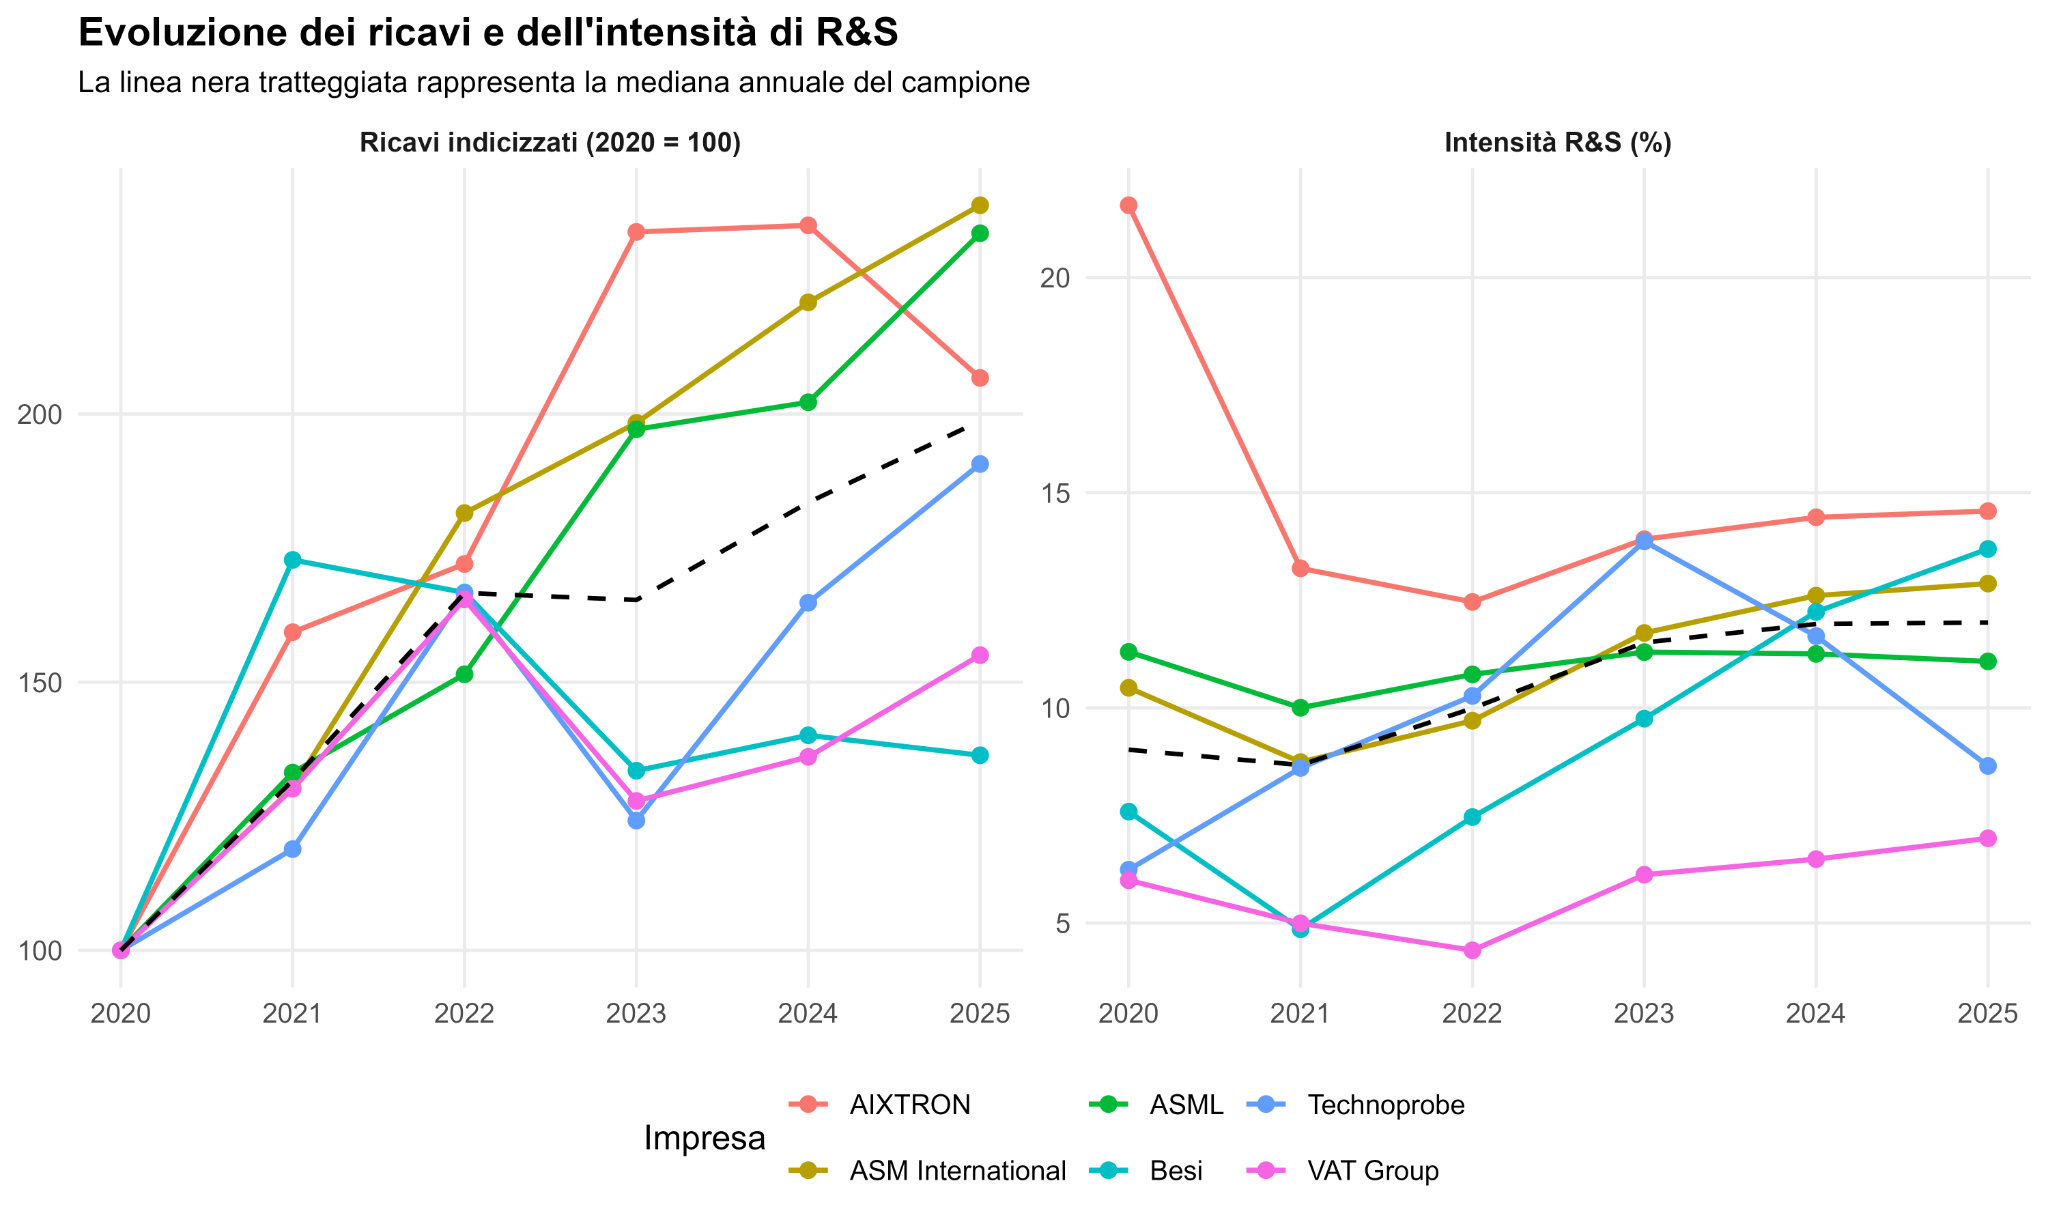
\includegraphics[width=0.94\textwidth]{01_crescita_innovazione.png}
\caption{Evoluzione dei ricavi e dell'intensità di R\&S}
\label{fig:crescita_innovazione}
\end{figure}

La Figura \ref{fig:crescita_innovazione} evidenzia una forte espansione complessiva dei ricavi, ma con traiettorie differenti. La mediana dei ricavi indicizzati passa da 100 nel 2020 a circa 167 nel 2022 e rimane sostanzialmente stabile nel 2023, per poi risalire fino a circa 199 nel 2025. ASM International e ASML mostrano le crescite cumulative più regolari e raggiungono a fine periodo valori prossimi rispettivamente a 239 e 234. AIXTRON registra una marcata accelerazione fino al 2023, seguita da una flessione nel 2025, mentre Besi e VAT Group evidenziano una crescita complessivamente più contenuta. Technoprobe presenta invece una traiettoria più discontinua, con una contrazione nel 2023 e un successivo recupero.

Il rallentamento osservato nel 2023 si inserisce in una fase di correzione più generale del ciclo dei semiconduttori. Dopo i livelli record raggiunti dagli investimenti produttivi nel 2022, la riduzione della domanda di chip e gli elevati livelli di scorte nei comparti consumer e mobile hanno determinato una contrazione degli investimenti in nuovi impianti \citep{semi2023}. Tale dinamica emerge anche nei risultati di Technoprobe, che nel 2023 attribuisce il calo dei ricavi alla contrazione del mercato di riferimento e agli elevati livelli di inventario detenuti dai clienti \citep{technoprobe2023h1}.

La successiva ripresa non appare tuttavia uniforme lungo la filiera. ASM International, ad esempio, è direttamente esposta alle tecnologie di deposizione utilizzate nei nodi più avanzati: nel 2024 la società ha registrato una forte domanda collegata alle architetture gate-all-around (GAA) e alle memorie ad alta larghezza di banda (HBM), individuando nell'intelligenza artificiale uno dei principali fattori di sostegno del mercato \citep{asm2024q3}. Besi opera invece nell'advanced packaging, segmento nel quale la crescita della domanda per soluzioni 2.5D e applicazioni destinate ai data center si accompagna a una maggiore debolezza di mercati tradizionali quali mobile, automotive e industriale \citep{besi2026}. La diversa esposizione ai segmenti tecnologici che guidano il recupero contribuisce quindi a spiegare perché la ripresa dei ricavi non avvenga con la stessa intensità e negli stessi anni per tutte le imprese.

Anche l'intensità di ricerca e sviluppo mostra una tendenza complessivamente crescente. La mediana del campione passa da circa il 9\% nel 2020 a circa il 12\% nel 2025. AIXTRON mantiene per gran parte del periodo una quota di R\&S superiore al benchmark, mentre ASM International e Besi mostrano un incremento progressivo dell'indicatore. Technoprobe raggiunge invece il valore massimo nel 2023 per poi ridurre l'incidenza della R\&S negli anni successivi.

Il profilo di AIXTRON evidenzia in particolare come un'elevata intensità innovativa non si traduca necessariamente in una crescita uniforme dei ricavi. La società è esposta principalmente ai semiconduttori composti e serve, tra gli altri, i mercati della power electronics e dell'optoelettronica. Nel 2025 la domanda nei segmenti GaN e SiC per applicazioni di potenza è rimasta debole, mentre le applicazioni optoelettroniche hanno beneficiato della crescente domanda di laser e soluzioni fotoniche per la trasmissione ad alta velocità dei dati \citep{aixtron2026}. La flessione dei ricavi osservata nell'ultimo anno può quindi essere letta anche alla luce della diversa dinamica dei mercati finali serviti. Nel complesso, l'aumento dell'intensità mediana di R\&S suggerisce inoltre che il rallentamento ciclico non abbia comportato una riduzione generalizzata dell'impegno innovativo.

\subsection{Marginalità e utilizzo degli asset}

Per valutare se l'espansione dimensionale sia stata accompagnata da un analogo miglioramento delle performance operative, vengono considerati il ROS e l'Asset Turnover. Il primo misura la quota di ricavi trasformata in risultato operativo, mentre il secondo esprime la capacità dell'impresa di generare ricavi attraverso gli asset impiegati.

\begin{figure}[H]
\centering
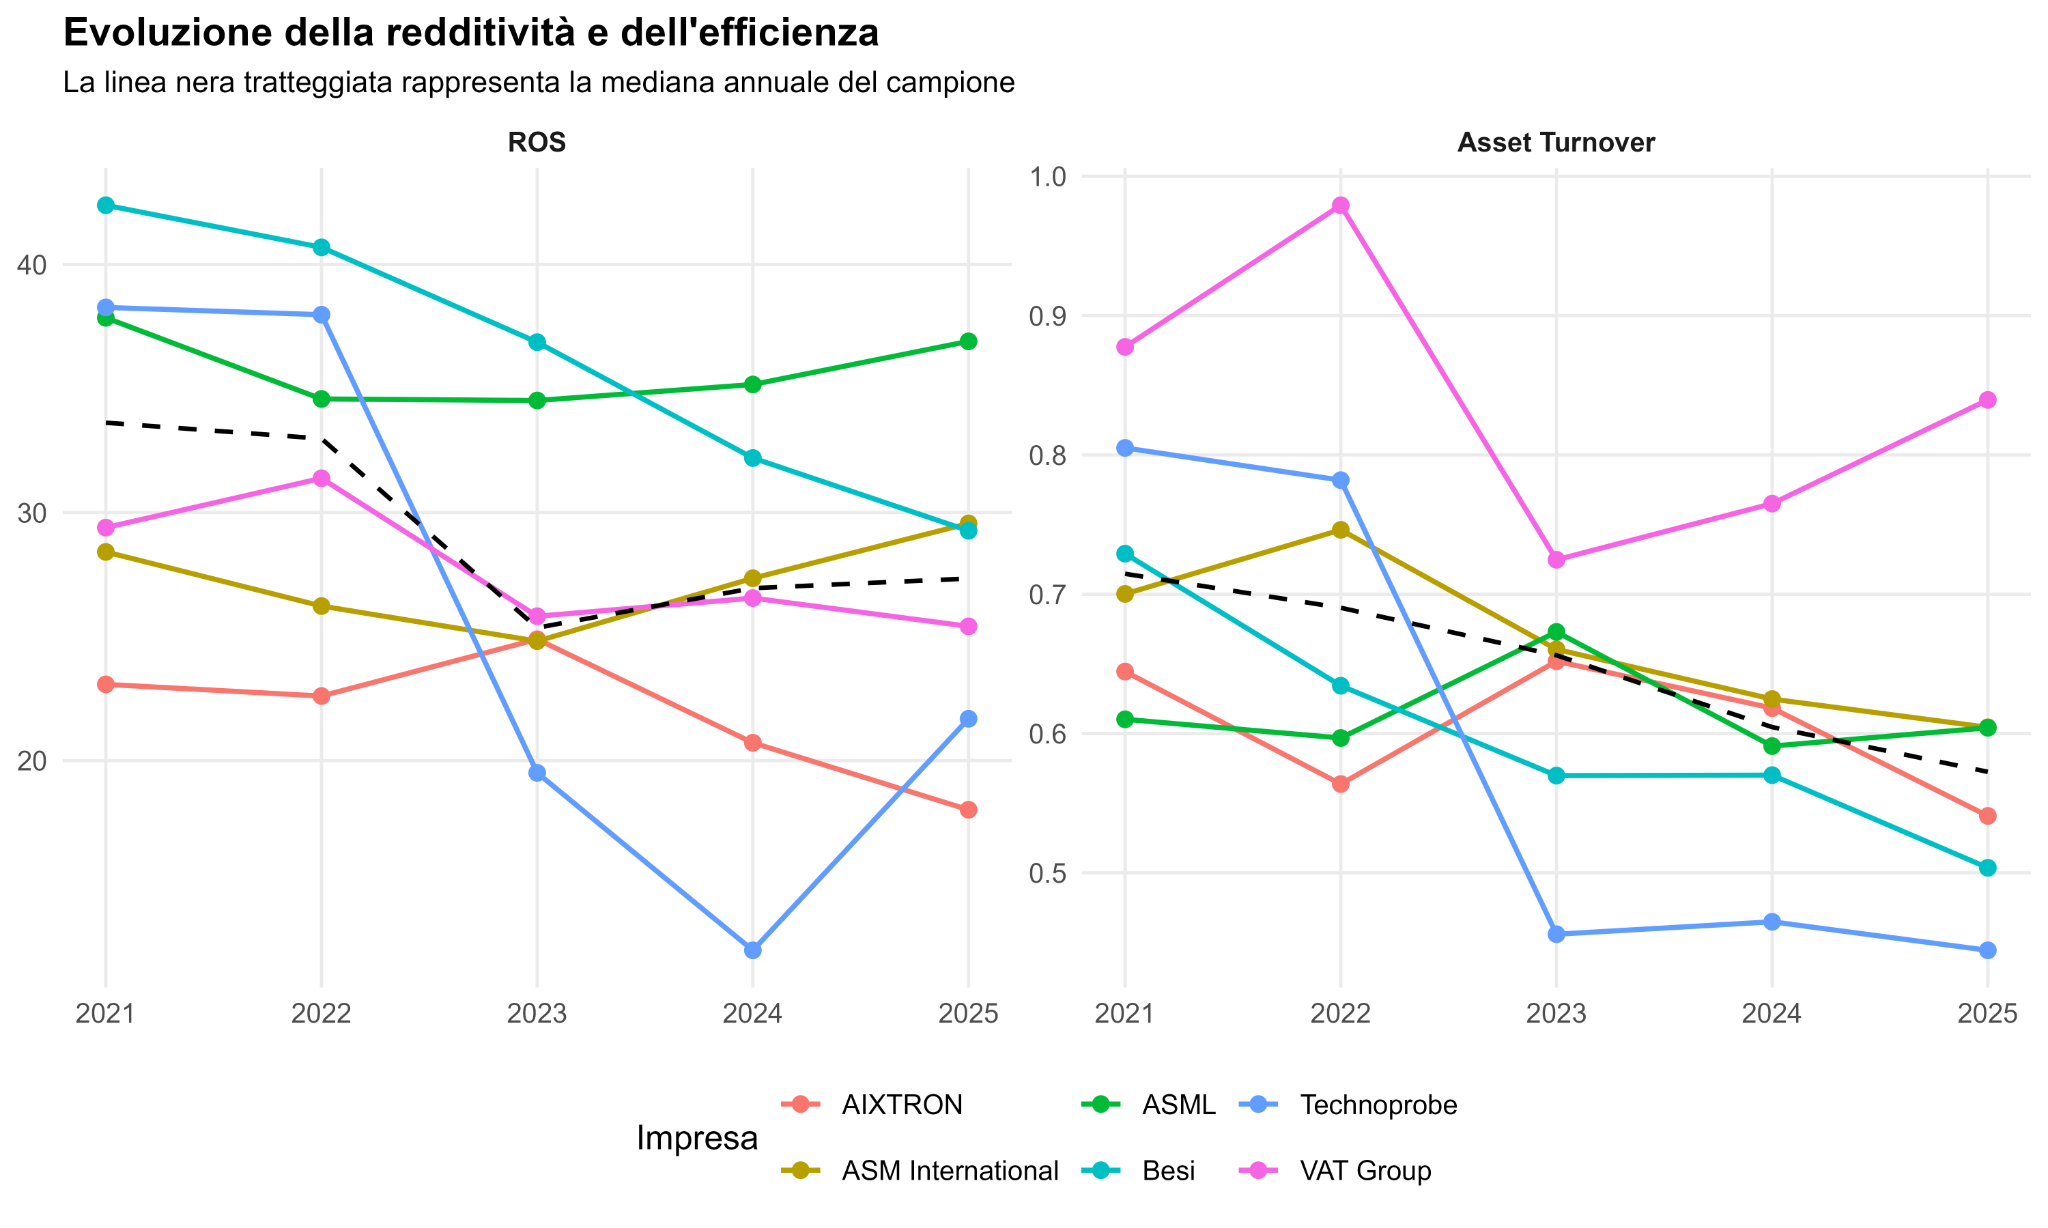
\includegraphics[width=0.94\textwidth]{02_redditivita_efficienza.png}
\caption{Evoluzione della redditività e dell'efficienza}
\label{fig:redditivita_efficienza}
\end{figure}

La Figura \ref{fig:redditivita_efficienza} mostra che la crescita osservata nei ricavi non si traduce in un miglioramento uniforme della redditività. Il ROS mediano si mantiene intorno al 33\% nel 2021--2022, scende a circa il 25\% nel 2023 e recupera solo parzialmente negli anni successivi, raggiungendo circa il 27\% nel 2025. ASML mantiene per tutto il periodo una redditività operativa superiore al benchmark e relativamente stabile. Besi parte da livelli ancora più elevati, ma mostra una progressiva riduzione del margine, mentre Technoprobe registra la variazione più marcata, passando da valori prossimi al 38\% nel 2021--2022 a circa il 12\% nel 2024, prima di recuperare nell'ultimo anno.

L'Asset Turnover presenta una riduzione più generalizzata: la mediana passa da circa 0,71 nel 2021 a 0,57 nel 2025. VAT Group mantiene i valori più elevati per quasi tutto il periodo, mentre Technoprobe mostra una forte riduzione a partire dal 2023. Il calo dell'indicatore segnala che, nel complesso, la crescita della base patrimoniale è stata più rapida della capacità di generare ricavi attraverso gli asset disponibili. Tale andamento non implica necessariamente un peggioramento dell'efficienza in senso assoluto, poiché può riflettere anche investimenti e ampliamenti della capacità destinati a sostenere la crescita futura.

Il caso di Technoprobe consente di leggere più chiaramente il legame tra ciclo di mercato, marginalità e utilizzo degli asset. Nel 2023 la riduzione della domanda e gli elevati livelli di inventario detenuti dai clienti hanno determinato una forte contrazione delle vendite. La minore attività produttiva ha ridotto l'assorbimento dei costi fissi, contribuendo alla compressione dei margini; contemporaneamente, la società ha scelto di mantenere la struttura produttiva e le risorse impiegate in previsione di una successiva ripresa dei volumi \citep{technoprobe2023h1}.

Nello stesso periodo Technoprobe ha continuato a sostenere gli investimenti produttivi e tecnologici e, nell'agosto 2023, ha acquisito Harbor Electronics, ampliando il proprio perimetro industriale nel settore dei circuiti stampati avanzati utilizzati nelle probe card \citep{technoprobe2024}. La contemporanea diminuzione del ROS e dell'Asset Turnover appare quindi coerente con una fase in cui i ricavi si sono ridotti mentre la capacità produttiva e la base di asset sono state in larga misura preservate e successivamente rafforzate. Il recupero dei ricavi osservato dal 2024 non determina infatti un immediato ritorno ai livelli di redditività e rotazione degli asset precedenti alla correzione.

Nel complesso, il confronto evidenzia una distinzione tra crescita dimensionale e performance operativa: le imprese che registrano la maggiore espansione dei ricavi non presentano necessariamente il miglioramento più marcato dei margini o della rotazione degli asset. Le differenti traiettorie riflettono quindi non soltanto l'andamento generale del mercato, ma anche il momento con cui i diversi segmenti della filiera attraversano le fasi di investimento, rallentamento e successivo recupero.

\subsection{Solidità patrimoniale e liquidità}

La struttura finanziaria viene analizzata attraverso l'autonomia finanziaria e il Current Ratio. Il primo indicatore misura l'incidenza del patrimonio netto sul totale dell'attivo, mentre il secondo consente di valutare l'equilibrio finanziario di breve periodo confrontando attività e passività correnti.

\begin{figure}[H]
\centering
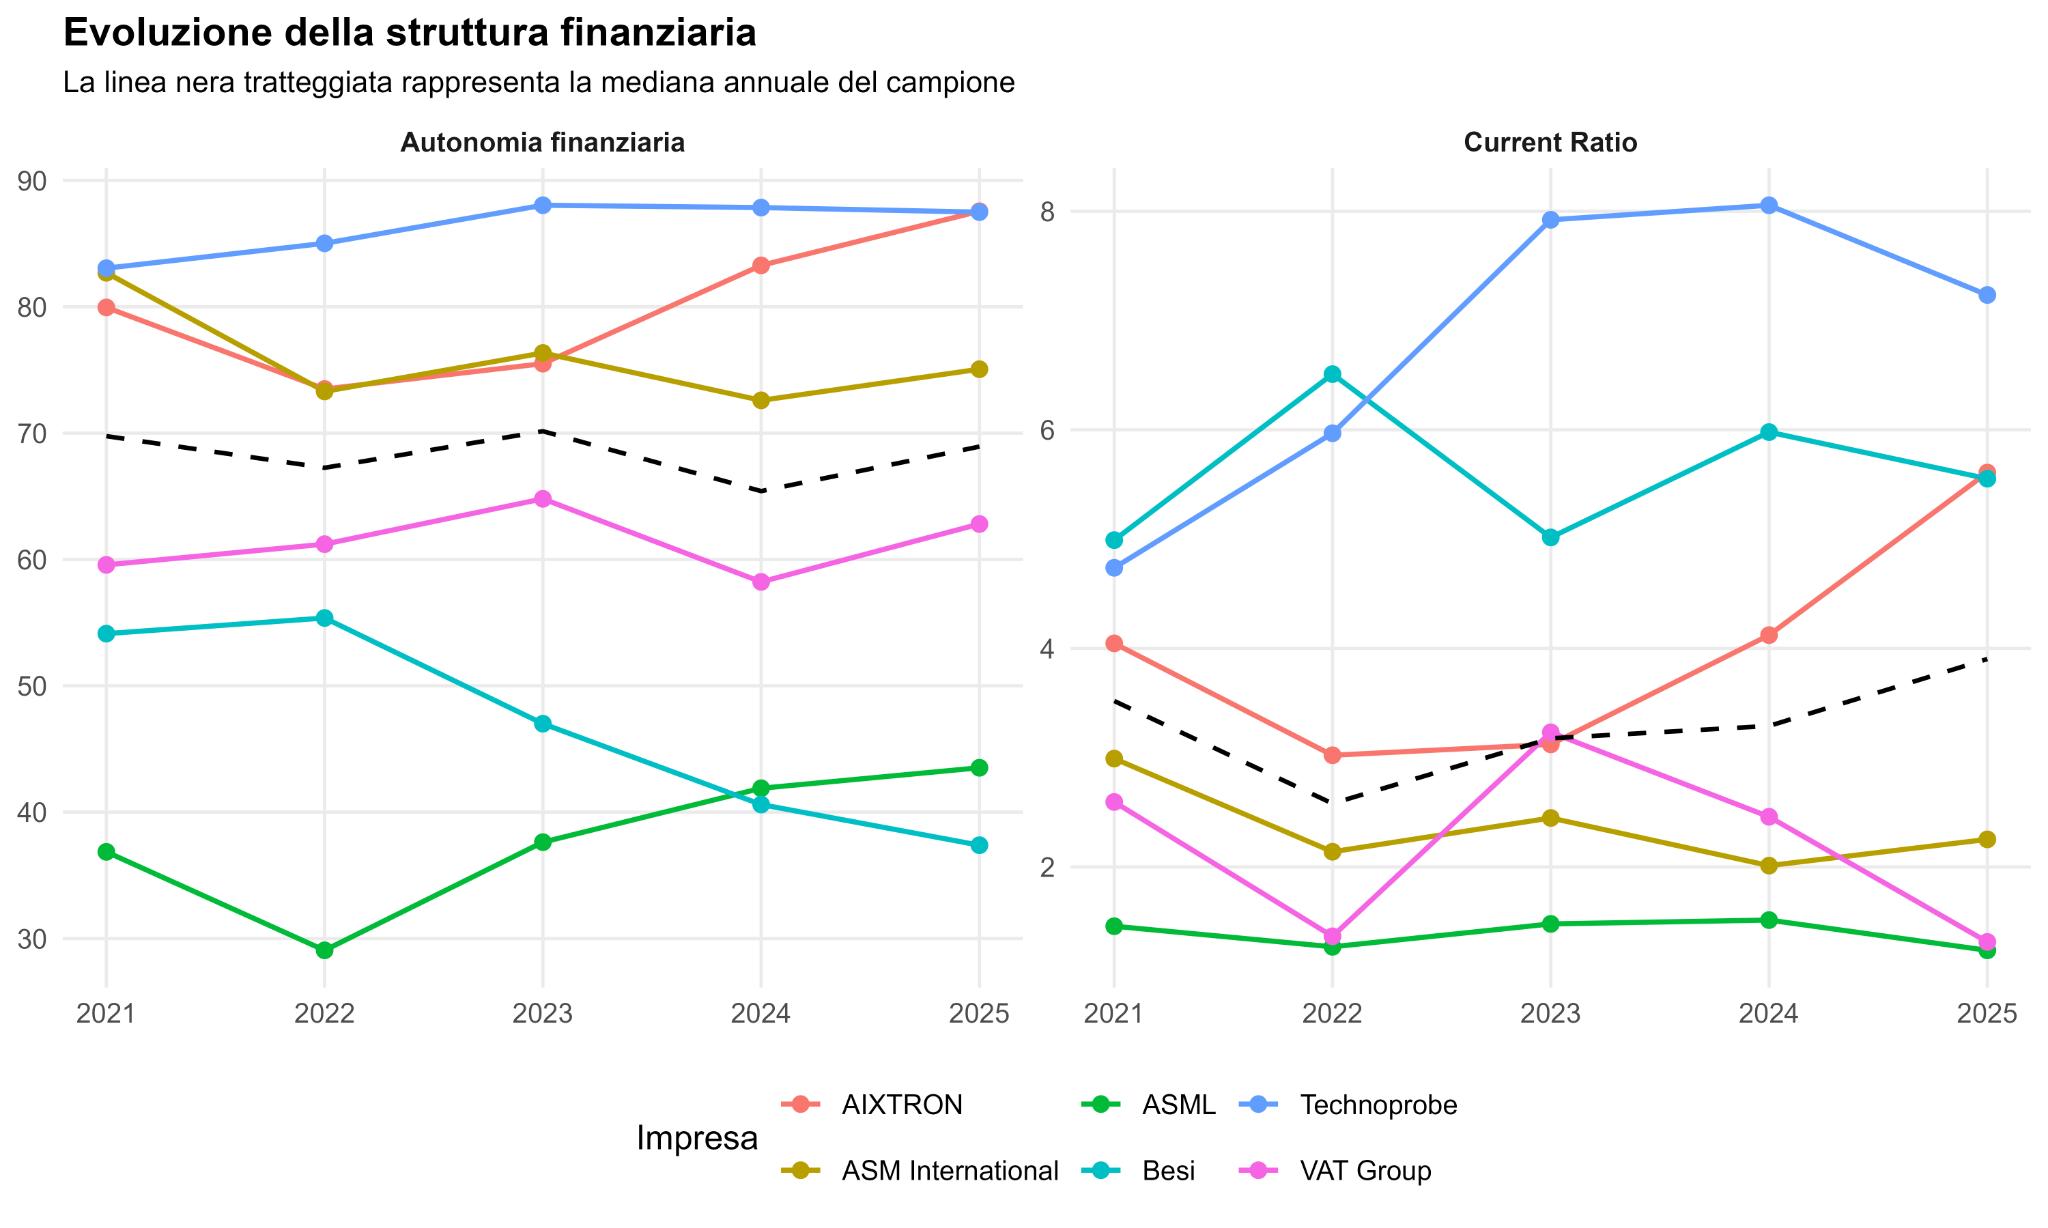
\includegraphics[width=0.94\textwidth]{03_struttura_finanziaria.png}
\caption{Evoluzione della struttura finanziaria}
\label{fig:struttura_finanziaria}
\end{figure}

La Figura \ref{fig:struttura_finanziaria} evidenzia profili finanziari nettamente differenziati. La mediana dell'autonomia finanziaria rimane complessivamente stabile, oscillando nel periodo tra circa il 65\% e il 70\%. Technoprobe presenta valori superiori all'80\% per l'intero periodo, mentre AIXTRON rafforza progressivamente la propria autonomia fino a raggiungere circa l'88\% nel 2025. Anche ASM International si mantiene stabilmente sopra il benchmark. ASML e Besi mostrano invece una minore incidenza del patrimonio netto sul totale dell'attivo, pur seguendo traiettorie differenti.

Le differenze risultano altrettanto evidenti nella liquidità. Il Current Ratio mediano scende da circa 3,5 nel 2021 a 2,6 nel 2022, per poi risalire progressivamente fino a circa 3,9 nel 2025. Technoprobe mantiene i valori più elevati nella parte finale del periodo, mentre Besi presenta anch'essa una liquidità ampiamente superiore al benchmark. ASML si colloca invece stabilmente su livelli inferiori alla mediana. In tutte le osservazioni il Current Ratio rimane comunque superiore a uno, indicando che le attività correnti risultano superiori alle passività correnti.

Il confronto mostra quindi che non emerge un unico profilo finanziario associato alle imprese con maggiore crescita o redditività. ASML, ad esempio, mantiene una redditività operativa tra le più elevate del campione pur presentando livelli di autonomia finanziaria e liquidità inferiori alla mediana. Technoprobe mostra invece una struttura patrimoniale particolarmente solida e un Current Ratio elevato, a fronte di una redditività che si riduce sensibilmente nel 2023--2024. Le diverse dimensioni della performance non coincidono pertanto in una graduatoria univoca, rendendo utile una successiva lettura congiunta attraverso l'Analisi in Componenti Principali.

\section{Profili competitivi e sintesi multidimensionale}

\subsection{Impostazione della PCA e capacità di sintesi}

Il benchmarking ha evidenziato come crescita, innovazione, redditività ed equilibrio finanziario non si muovano necessariamente nella stessa direzione. Per osservare congiuntamente queste dimensioni viene applicata un'Analisi in Componenti Principali (PCA), che consente di sintetizzare l'informazione contenuta negli indicatori originari in un numero più ridotto di componenti.

L'analisi è condotta sulle 30 osservazioni impresa--anno del periodo 2021--2025 e considera cinque variabili: crescita annuale dei ricavi, ROS, intensità di ricerca e sviluppo, Asset Turnover e autonomia finanziaria. Prima dell'applicazione della PCA, gli indicatori sono stati standardizzati, così da eliminare l'influenza delle differenti unità di misura e rendere confrontabile il loro contributo alla costruzione delle componenti.

\begin{table}[H]
\centering
\caption{Autovalori e varianza spiegata dalle componenti principali}
\small
\begin{tabular}{lrrr}
\toprule
\textbf{Componente} & \textbf{Autovalore} & \textbf{Varianza (\%)} & \textbf{Cumulata (\%)} \\
\midrule
PC1 & 2,309 & 46,2 & 46,2 \\
PC2 & 1,324 & 26,5 & 72,6 \\
PC3 & 0,784 & 15,7 & 88,3 \\
PC4 & 0,312 & 6,2 & 94,6 \\
PC5 & 0,271 & 5,4 & 100,0 \\
\bottomrule
\end{tabular}
\end{table}

Le prime due componenti presentano un autovalore superiore a uno e spiegano congiuntamente il 72,6\% della variabilità complessiva. La rappresentazione nel piano formato da PC1 e PC2 conserva quindi una quota ampia dell'informazione contenuta nei cinque indicatori e viene utilizzata per la lettura sintetica dei profili aziendali.

\subsection{Interpretazione delle componenti}

Per attribuire un significato economico alle due dimensioni trattenute, si osservano le associazioni tra gli indicatori originari e le componenti principali.

\begin{table}[H]
\centering
\caption{Associazione delle variabili originarie con PC1 e PC2}
\small
\begin{tabular}{lrr}
\toprule
\textbf{Variabile} & \textbf{PC1} & \textbf{PC2} \\
\midrule
Crescita ricavi ($\Delta$RIC) & -0,471 & 0,481 \\
ROS & -0,765 & -0,472 \\
Intensità R\&S & 0,809 & -0,227 \\
Asset Turnover (AT) & -0,778 & 0,438 \\
Autonomia finanziaria (AF) & 0,492 & 0,792 \\
\bottomrule
\end{tabular}
\end{table}

La prima componente, che spiega il 46,2\% della varianza, contrappone soprattutto l'intensità di ricerca e sviluppo e, in misura minore, l'autonomia finanziaria, alla redditività operativa e alla capacità di generare ricavi attraverso gli asset. Valori positivi di PC1 risultano quindi associati a una maggiore intensità di R\&S, mentre ROS e Asset Turnover presentano associazioni negative elevate.

La seconda componente spiega il 26,5\% della varianza ed è associata soprattutto all'autonomia finanziaria, alla quale si affiancano la crescita dei ricavi e l'Asset Turnover; sul lato opposto si colloca principalmente il ROS. PC2 può quindi essere letta soprattutto come una dimensione di solidità patrimoniale e dinamica di crescita. Il segno delle componenti è convenzionale: l'interpretazione riguarda le opposizioni tra variabili e non una scala automatica tra posizioni migliori e peggiori.

\subsection{Posizionamento e traiettorie delle imprese}

Il piano fattoriale consente di leggere contemporaneamente la posizione delle imprese e la loro evoluzione nel tempo. Le traiettorie vengono interpretate collegando gli spostamenti nel piano ai risultati emersi nel benchmarking, senza attribuire alle componenti un significato di graduatoria.

\begin{figure}[H]
\centering
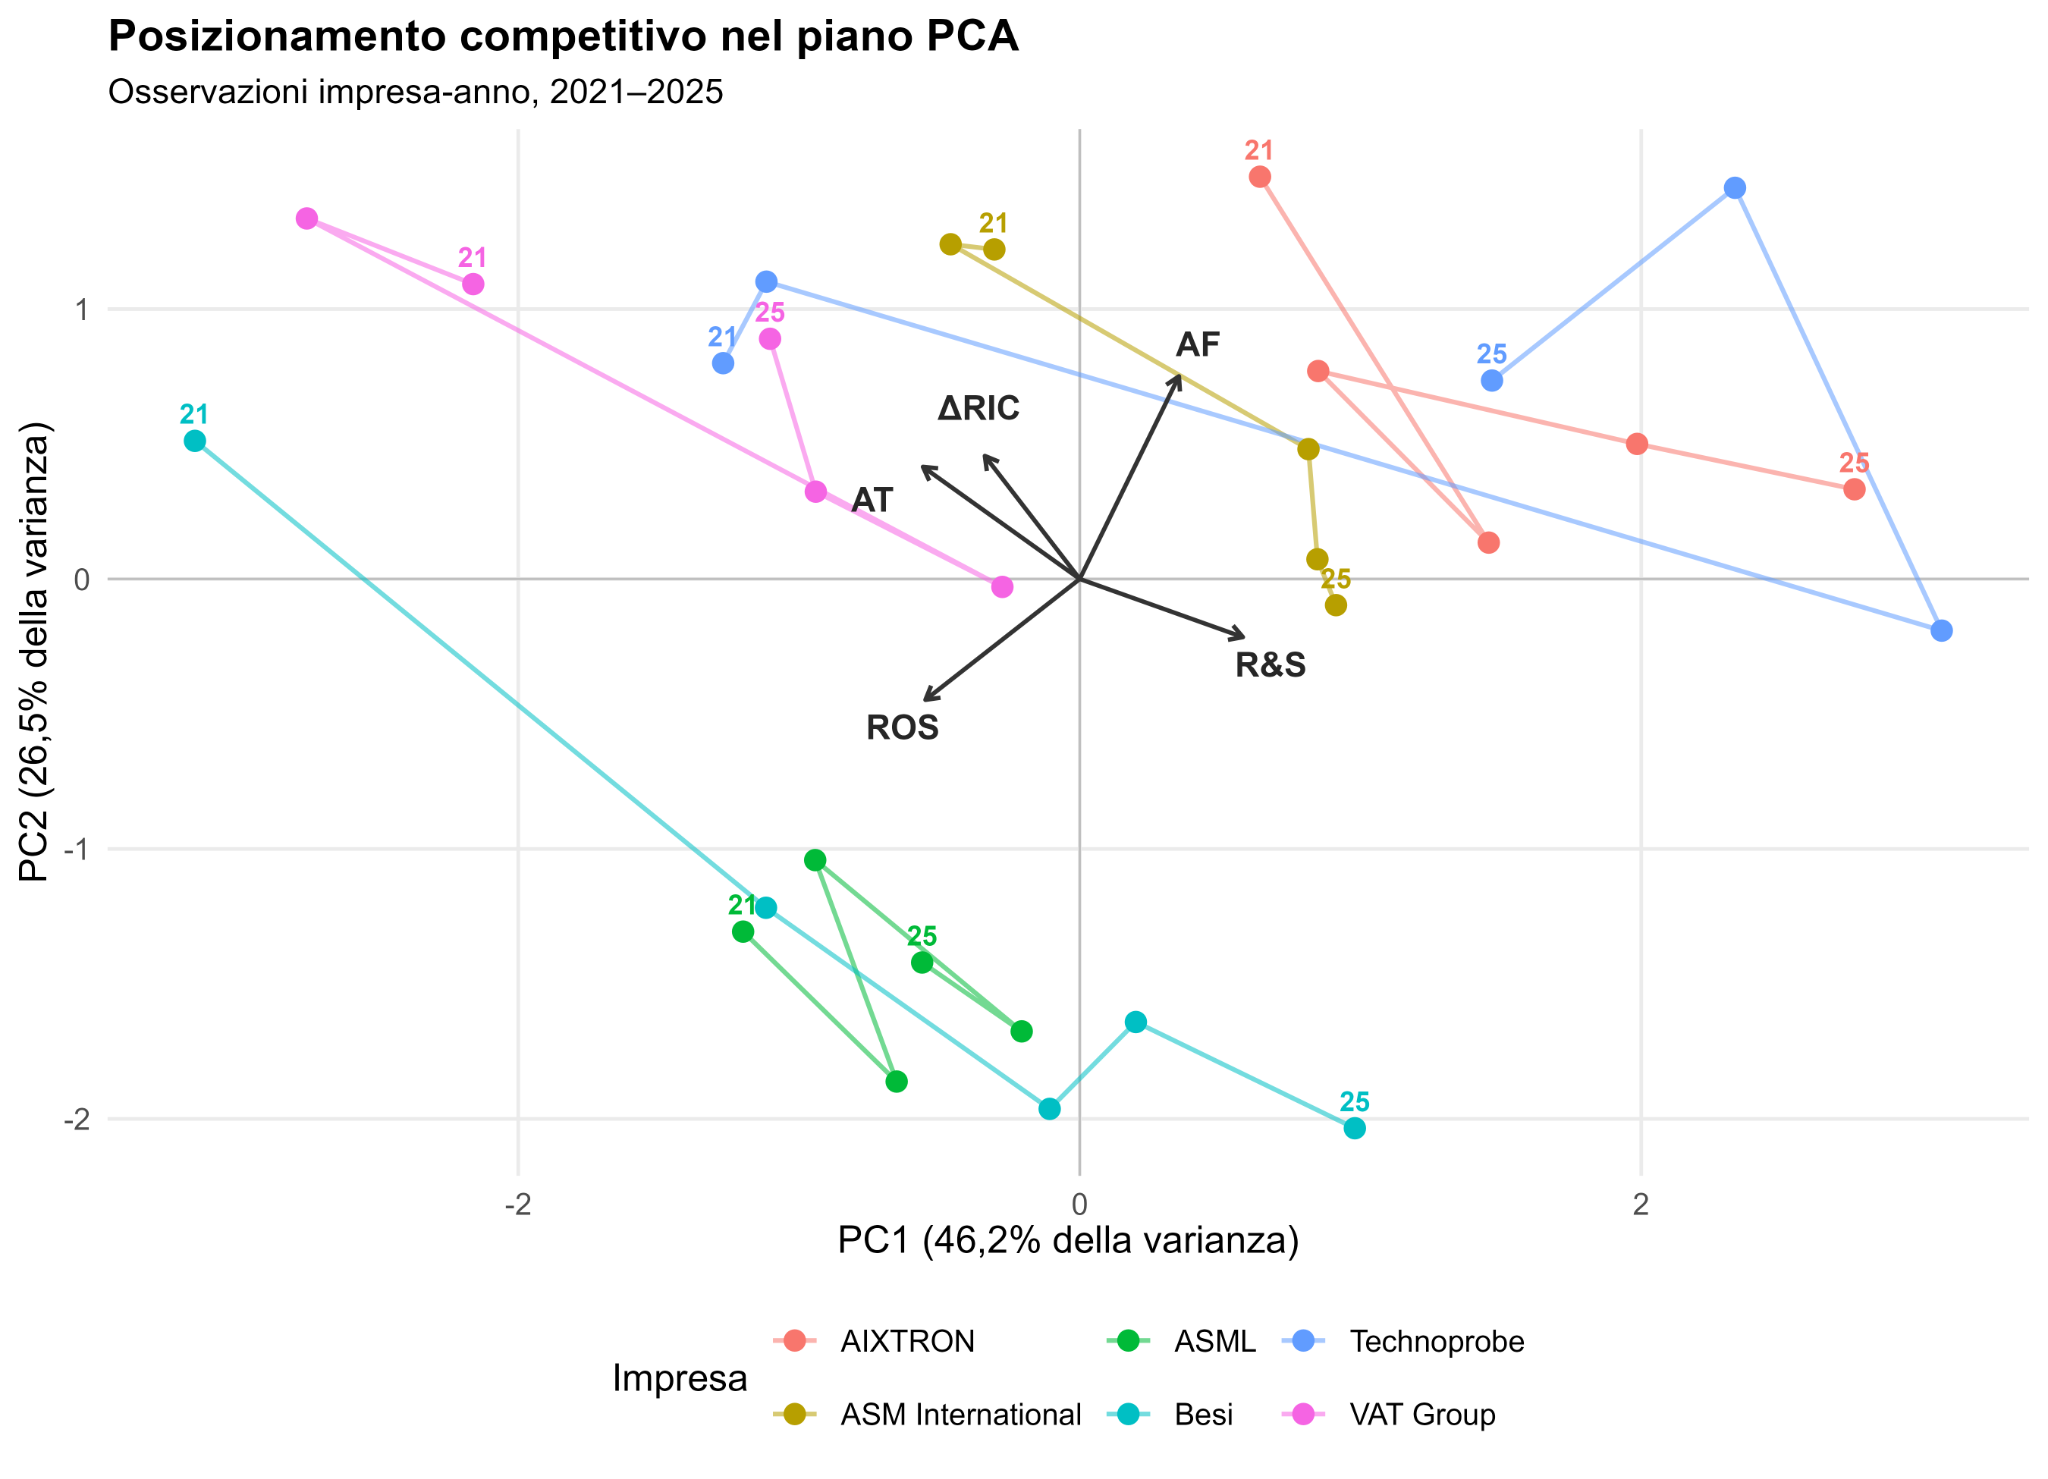
\includegraphics[width=0.92\textwidth]{04_pca_mappa_competitiva.png}
\caption{Posizionamento competitivo delle imprese nel piano PCA}
\label{fig:pca}
\end{figure}

La Figura \ref{fig:pca} mostra come le differenze osservate nel benchmarking si riflettano nel posizionamento congiunto delle imprese. L'origine del piano rappresenta il profilo medio delle osservazioni standardizzate dell'intero campione e non coincide con il benchmark mediano annuale utilizzato nei grafici precedenti.

\paragraph{AIXTRON e ASML.}
AIXTRON si colloca per l'intero periodo nel lato positivo della prima componente e si sposta ulteriormente verso destra nel 2025. Tale posizione è coerente con l'elevata intensità di ricerca e sviluppo e con la forte autonomia finanziaria, alle quali si accompagnano negli anni più recenti livelli più contenuti di redditività e rotazione degli asset. ASML presenta un profilo quasi speculare e rimane stabilmente nel quadrante inferiore sinistro: il suo posizionamento è associato soprattutto al ROS persistentemente elevato, mentre la minore autonomia finanziaria contribuisce ai valori negativi della seconda componente. Il confronto mette quindi in evidenza due configurazioni competitive differenti, una maggiormente caratterizzata dall'intensità innovativa e dalla solidità patrimoniale e l'altra dalla redditività operativa.

\paragraph{Besi.}
Besi mostra uno degli spostamenti più ampi nel piano fattoriale. Tra il 2021 e il 2025 l'impresa si muove dal quadrante superiore sinistro verso quello inferiore destro, passando da valori fortemente negativi a positivi su PC1 e, contemporaneamente, da valori positivi a fortemente negativi su PC2. Lo spostamento lungo PC1 è coerente con il progressivo aumento dell'intensità di R\&S e con la riduzione del ROS e dell'Asset Turnover; il movimento verso valori più bassi di PC2 riflette soprattutto il rallentamento della crescita e la diminuzione dell'autonomia finanziaria. La traiettoria descrive quindi una trasformazione del profilo dell'impresa, più che un semplice miglioramento o peggioramento complessivo.

\paragraph{Technoprobe.}
Technoprobe presenta una traiettoria altrettanto dinamica. Nel 2021--2022 si colloca nella parte superiore sinistra del piano, coerentemente con livelli elevati di ROS e Asset Turnover e con una forte autonomia finanziaria. Nel 2023 il profilo cambia nettamente: la crescita dei ricavi diventa negativa, il ROS scende da circa il 38\% al 19,5\% e l'Asset Turnover passa da 0,78 a circa 0,46, mentre l'intensità di R\&S raggiunge il valore massimo del periodo. Nel 2024 la redditività si riduce ulteriormente; nel 2025 la traiettoria torna invece parzialmente verso il centro, con un recupero del ROS e una struttura patrimoniale ancora molto solida. Il percorso evidenzia quindi una fase di forte discontinuità seguita da segnali di riequilibrio nell'ultimo anno.

Nel complesso, la PCA conferma che le imprese non possono essere ordinate secondo una graduatoria univoca. Il posizionamento dipende dalla combinazione tra crescita, innovazione, redditività, utilizzo degli asset e solidità finanziaria: società collocate in aree differenti del piano possono quindi presentare punti di forza su dimensioni diverse.

\section{Conclusioni}

Nel periodo 2021--2025 il campione mostra una forte espansione complessiva, interrotta dalla correzione ciclica del 2023 e seguita da una ripresa selettiva. La crescita dei ricavi si accompagna a un'intensità di ricerca e sviluppo mediamente crescente, ma non produce effetti uniformi su redditività e utilizzo degli asset: il ROS recupera solo in parte dopo il 2023, mentre l'Asset Turnover si riduce progressivamente.

Le differenze tra le imprese risultano quindi sostanziali. ASML e ASM International mostrano le traiettorie di crescita più regolari, AIXTRON combina elevata intensità innovativa e forte autonomia finanziaria, mentre Besi e Technoprobe evidenziano le trasformazioni più marcate del proprio profilo. La PCA, che sintetizza il 72,6\% della variabilità nelle prime due componenti, conferma che non esiste un unico modello di successo: redditività, innovazione, crescita e solidità finanziaria tendono a concentrarsi in combinazioni differenti.

Nel contesto della crescente domanda di capacità di calcolo e delle applicazioni di intelligenza artificiale, il principale risultato è quindi la natura selettiva dell'evoluzione della filiera. I benefici della ripresa emergono con tempi e intensità diversi a seconda delle tecnologie e dei mercati finali serviti. Il posizionamento competitivo delle imprese analizzate dipende pertanto dalla capacità di combinare specializzazione tecnologica, innovazione e sostenibilità economico-finanziaria lungo fasi differenti del ciclo dei semiconduttori.

\begin{thebibliography}{99}
\small

\bibitem[SEMI(2023)]{semi2023}
SEMI (2023), \textit{2024 Global Fab Equipment Spending Recovery Expected After 2023 Slowdown, SEMI Reports}. Disponibile su: \url{https://www.semi.org/en/news-media-press-releases/semi-press-releases/2024-globaL-fab-equipment-spending-recovery-expected-after-2023-slowdown-semi-reports}.

\bibitem[Technoprobe(2023)]{technoprobe2023h1}
Technoprobe (2023), \textit{Interim Condensed Consolidated Financial Statements as at 30 June 2023}. Disponibile su: \url{https://www.technoprobe.com/wp-content/uploads/2023/08/ENG-Fascicolo-Technoprobe-SpA-30.06.2023.pdf}.

\bibitem[ASM International(2024)]{asm2024q3}
ASM International (2024), \textit{Q3 2024 Investor Presentation}. Disponibile su: \url{https://www.asm.com/downloads/presentations-other/2024-q3-investor-presentation}.

\bibitem[Besi(2026)]{besi2026}
BE Semiconductor Industries (2026), \textit{Q4-25 and Full Year 2025 Results}. Disponibile su: \url{https://www.besi.com/investor-relations/press-releases/details/be-semiconductor-industries-nv-announces-q4-25-and-full-year-2025-results/}.

\bibitem[AIXTRON(2026)]{aixtron2026}
AIXTRON (2026), \textit{AIXTRON with robust results in a soft market environment}. Disponibile su: \url{https://www.aixtron.com/en/investors/AIXTRON%20with%20robust%20results%20in%20a%20soft%20market%20environment_n13896}.

\bibitem[Technoprobe(2024)]{technoprobe2024}
Technoprobe (2024), \textit{Annual Financial Report 2023}. Disponibile su: \url{https://www.technoprobe.com/wp-content/uploads/2024/03/xTechnoprobe-SpA-ENG_RELAZIONE-ANNUALE-2023-FASCICOLO-COMPLETO-1.pdf}.

\end{thebibliography}

\end{document}
